\chapter{Validation in liquid jet in crossflow}
	\label{ch6:jicf_lgs_simulations}


%Describe here all our results from the lagrangian simulations:
%
%\begin{itemize}
%
%	\item Effects of applying full workflow: w/wo ALM, w/wo secondary atomization ...
%	
%	\item Mesh convergence study: specify it
%	
%	\item Validation with experiments
%	
%	\item Mass conservation issues: lagrangian tracking, etc. 
%	
%
%\end{itemize}


\section{Introduction}

This chapter presents results from lagrangian simulations performed with the SLI models described in Chapter \ref{ch4:sli_development}. The test case used is the academic JICF of \citeColor[becker_breakup_2002], for which resolved simulations of the atomization process were detailed in Chapter \ref{ch5:jicf_resolved_simulations}. Data for these computations are used to build the injectors in order to run dispersed phase simulations in the same configuration, which are shown to be less computationally expensive than the resolved ones. \hl{...}


\section{Computational setup}

The geometry replicating the experimental test bench is the same than the one used for the resolved simulations, depicted in Figure \ref{fig:numerical_setup_maquette_JICF_DLR}. The operating points simulated are the ones from Table \ref{tab:jicf_operating_conditions}. Regarding the mesh employed, it was shown in $\S$\ref{sec:ch5_initial_conditions} that an element size of $\Delta x = 0.5$ mm allows to transport the estimated turbulence in these cases. Nevertheless, the simulations from Chapter \ref{ch5:jicf_resolved_simulations} use a mesh with this cell size only inside the plenum upstream and around the injector, while downstream the injector the mesh size is enlarged since there is no liquid at this region. This mesh was shown in Figure \ref{fig:jicf_dlr_mesh}. In the lagrangian simulations performed in this chapter, injection is performed at the sampling planes downstream the injector \hl{shown in Chapter }\ref{ch5:jicf_resolved_simulations}, and the region of interest extends up to a location at $x = 80$ mm downstream the injector since this is where validation with the experimental results of \citeColor[becker_breakup_2002] can be performed. Therefore, lagrangian simulations use a baseline cell size of $\Delta x = 0.5$ mm in the plenum from the gaseous inlet up to $x = 85$ mm downstream the injector. In this way, turbulence can be transported from the gaseous inlet  up to the experimental validation plane. \hl{The mesh used, shown in Figure} \ref{fig:jicf_dlr_mesh_LGS}, is composed of \textbf{XX} elements, being therefore larger than the baseline mesh employed for the resolved simulations. However, in the dispersed phase simulations there is no Adaptive Mesh Refinement being performed, and therefore the number of mesh elements stays constant in all simulations. The lagrangian point-particle equations employed to model the dispersed phase are described in $\S$\textbf{XX}.

\begin{figure}[h!]
	\centering
	\includeinkscape[inkscapelatex=true,scale=0.8]{./part2_developments/figures_ch6_lagrangian_JICF/jicf_mesh_LGS}
	\caption{Mesh employed for LGS simulations. \hl{CHANGE WHEN READY}}
	\label{fig:jicf_dlr_mesh_LGS}
\end{figure}

%\section{Evaporation phenomena}
%
%\textbf{Note: this analysis could perfectly be in the previous chapter}.
%
%As indicated in Table \ref{tab:jicf_operating_conditions}, the temperatures of both liquid kerosene and gaseous air are low (290 and 288 K respectively) and there is not direct evaporation of fuel. Nevertheless, some evaporation can occur at ambient temperature if the vapour pressure of the liquid is lower than the ambient pressure. In the experiments, the ambient pressure is $p_g = 6$ bar, while the vapour pressure of kerosene at $288$ K is $p_{vap} = 0.003$ bar \citepColor[shepherd_flash_2000]. Therefore, evaporation might be possible.
%
%It is tested that ... Two characteristic times are used in the low We case (since the lowest velocity is found there, and the droplets take more time to reach the validation plane at 80 mm)/
%
%\begin{itemize}
%
%	\item The time that a droplet takes to reach the plane x = 80 mm. From the SPS results in $\S$\textbf{??} (or Table \textbf{??}), the first droplets at x = 10 mm are obtained at $t_{resolv} = 0.3$ ms after injection. Then, the first droplets injected at this location in the lagrangian simulations reach the validation plane after $t_\mathrm{lagr} = $ ms. Hence, a characteristic time defined as the :
%	
%	\begin{equation}
%	\tau_{validation} = t_{resolv}  + t_\mathrm{lagr}
%	\end{equation}
%	
%	\item Evaporation time rate is used by means of the $d^2$ law. This law that the square of the droplet's diameter diminishes linearly with time:
%	
%	\begin{equation}
%	\label{eq:d2_law}
%	d^2 \left( \right) = d_0^2 - K t
%	\end{equation}
%	
%	
%	where $K$ is the evaporation rate and $d_0$ the initial diameter of the droplet. The value K ... (see 2006 Ghassemi).
%	
%	
%	\text{NAH}. The evolution in diameter after a given time $t$ can then be obtained as:
%	
%	\begin{equation}
%	\Delta d^2 = d_0^2 - d^2 \left( \right) = K t
%	\end{equation}
%	
%
%\end{itemize}

\section{Experimental results from literature}

The study from \citeColor[becker_breakup_2002] reports results on the droplets average size SMD and the liquid volume fluxes in the plane $x = 80$  mm perpendicular to the crossflow. In the resolved simulations of Chapter \ref{ch5:jicf_resolved_simulations} the liquid spray could not reach this location: the increase in mesh size due to a continuous liquid injection and formation of droplets due to atomizatio yielded computations unfeasible if liquid was allowed to travel too far downstream, and hence the liquid domain was restricted up to $x = 10, 15$ mm for the fine and coarse resolutions respectively. This limitation does not apply in the dispersed phase simulations, which can be transported up to the outlet of the domain due to their lower cost compared to the resolved ones. Therefore, the dispersed phase simulations will be compared to the experimental results presented at 80 mm.

Experiments results from PDA measurements can be found in the articles \citeColor[becker_breakup_2002] and \citeColor[rachner_modelling_2002]. Among those, quantitative maps of SMD and volume flux are given, which are shown in Figure \ref{fig:maps_Becker_expe_results}. For both operating points, the volume flux shows a circumferential pattern where the largest flux is located at the center and is reduced radially. Most of the fuel is then located at the center of the spray plume, which is a common feature in liquid jets in crossflow \citepColor[wu_spray_1998]. The maximum value of volume flux is lower for the low Weber case than in the high Weber one, which is expected since the injected liquid mass flow rate is lower for the former than for the later to keep the same momentum flux ratio $q$ in both cases, as Table \ref{tab:jicf_operating_conditions} shows. Regarding the $SMD$, both maps show a ballistic, layered profile where the largest droplets are located in the top part of the spray. This is due to the higher inertia of the biggest droplets produced, which penetrate further than the smallest ones \citepColor[wu_breakup_1997]. In general, $SMD$ values are larger in the low Weber case since the dynamic pressure (or equivalently, the gaseous velocity) is lower, and the size of the droplets produced were found to be highly dependent on this parameter \citepColor[becker_breakup_2002].


%\begin{figure}[h!]
%\flushleft
%\begin{subfigure}[b]{0.4\textwidth}
%	\centering
%   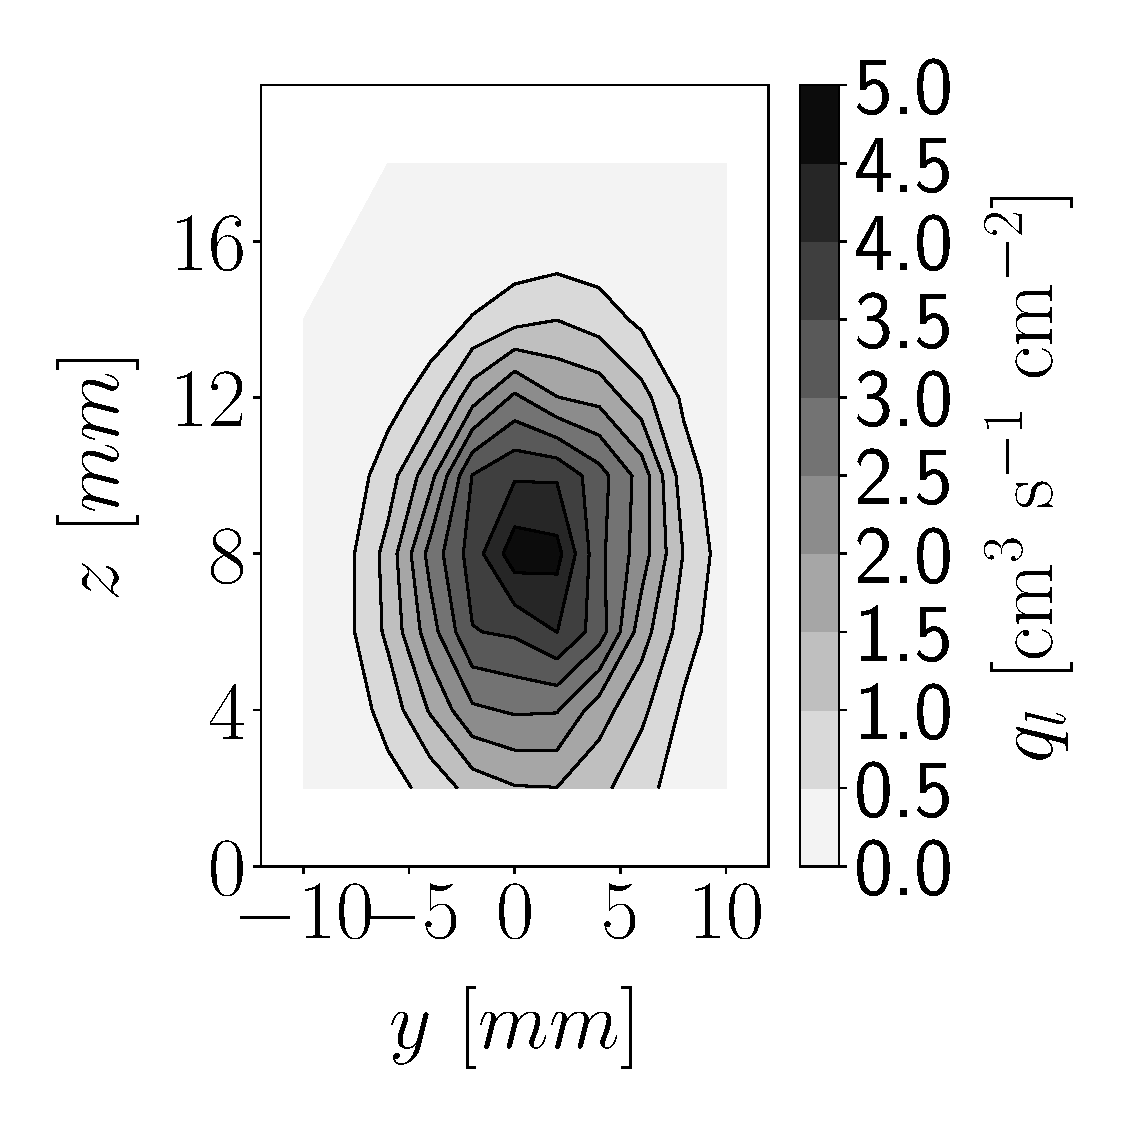
\includegraphics[scale=0.2]{./part2_developments/figures_ch6_lagrangian_JICF/expe_results/map_flux_UG100}
%   \hspace{-0.1in}
%   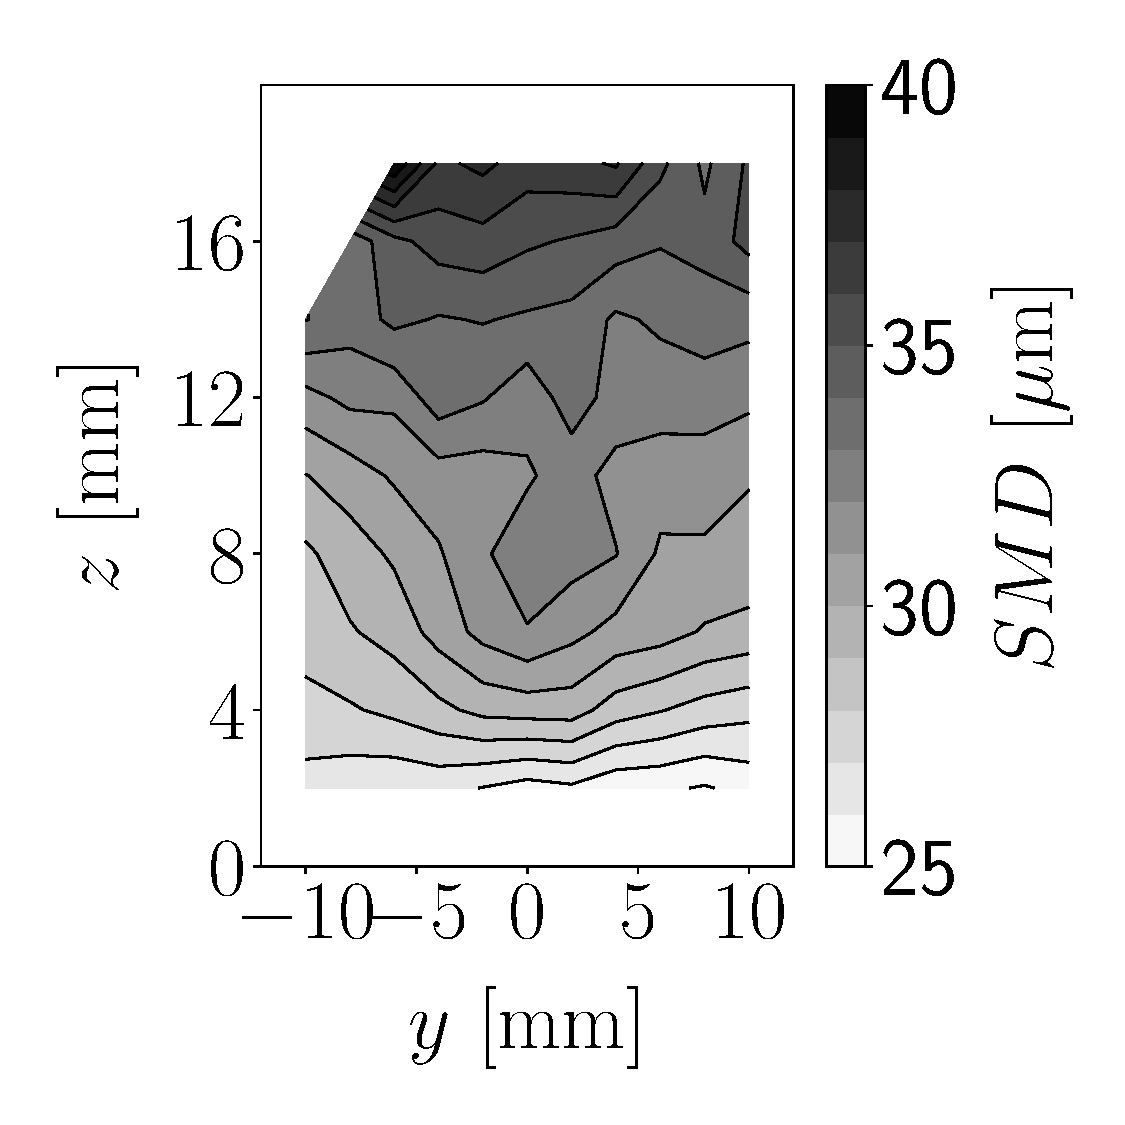
\includegraphics[scale=0.2]{./part2_developments/figures_ch6_lagrangian_JICF/expe_results/map_SMD_UG100}
%   \caption{Low Weber number operating point.}
%   %\label{} 
%\end{subfigure}
%\begin{subfigure}[b]{0.4\textwidth}
%	\flushleft
%   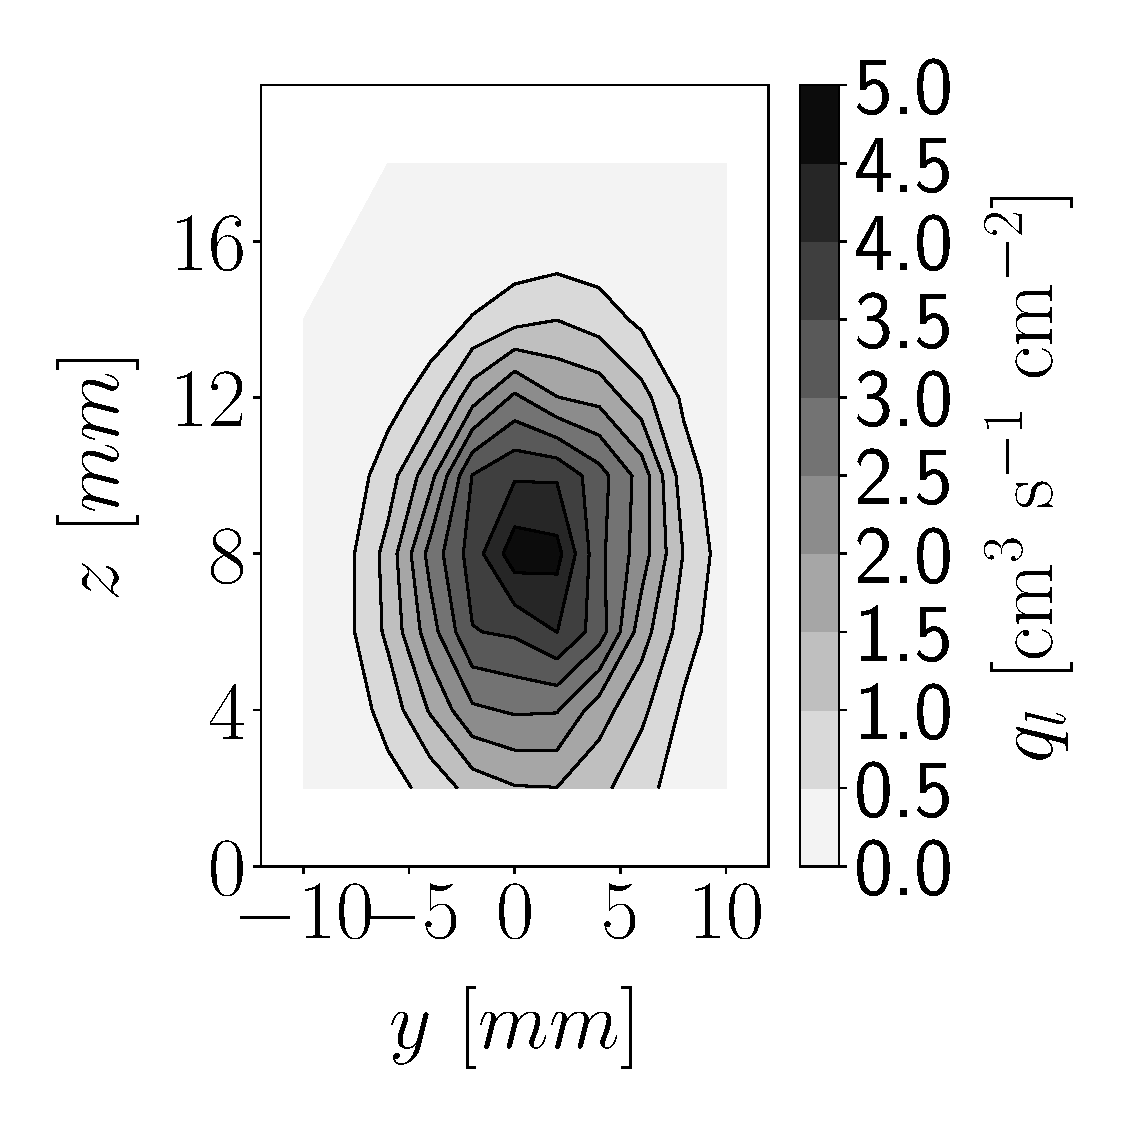
\includegraphics[scale=0.1]{./part2_developments/figures_ch6_lagrangian_JICF/expe_results/map_flux_UG100}
%   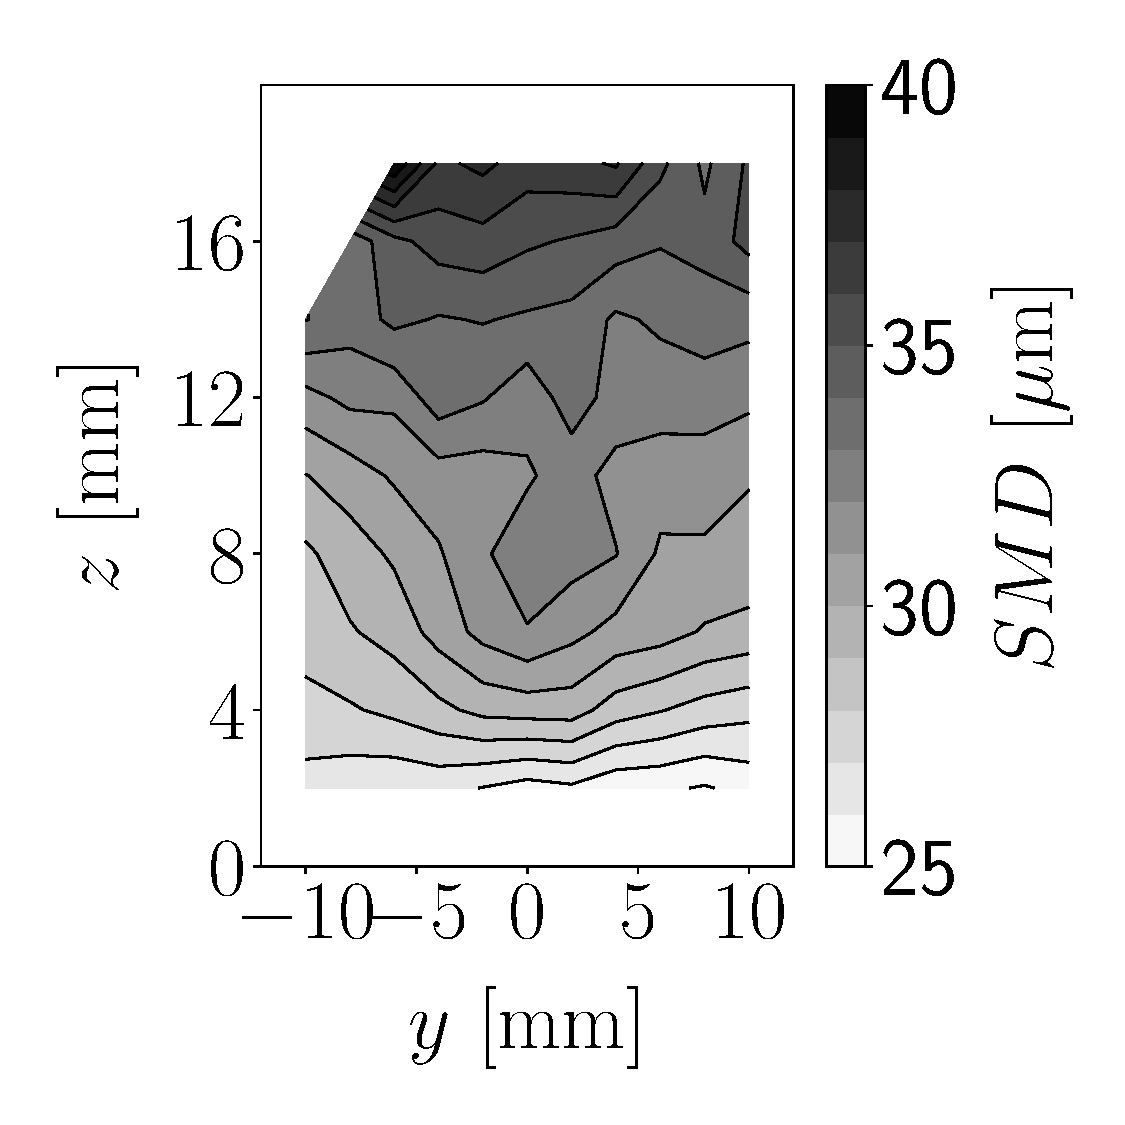
\includegraphics[scale=0.1]{./part2_developments/figures_ch6_lagrangian_JICF/expe_results/map_SMD_UG100}
%   \caption{High Weber number operating point.}
%   %\label{} 
%\end{subfigure}
%\caption{SMD and volume flux maps obtained experimentally by \citeColor[becker_breakup_2002] at a location $x = 80$ mm downstream the liquid injector.}
%\label{fig:maps_Becker_expe_results}
%\end{figure}


\begin{figure}[h!]
\flushleft
\begin{subfigure}[b]{0.45\textwidth}
	\flushleft
   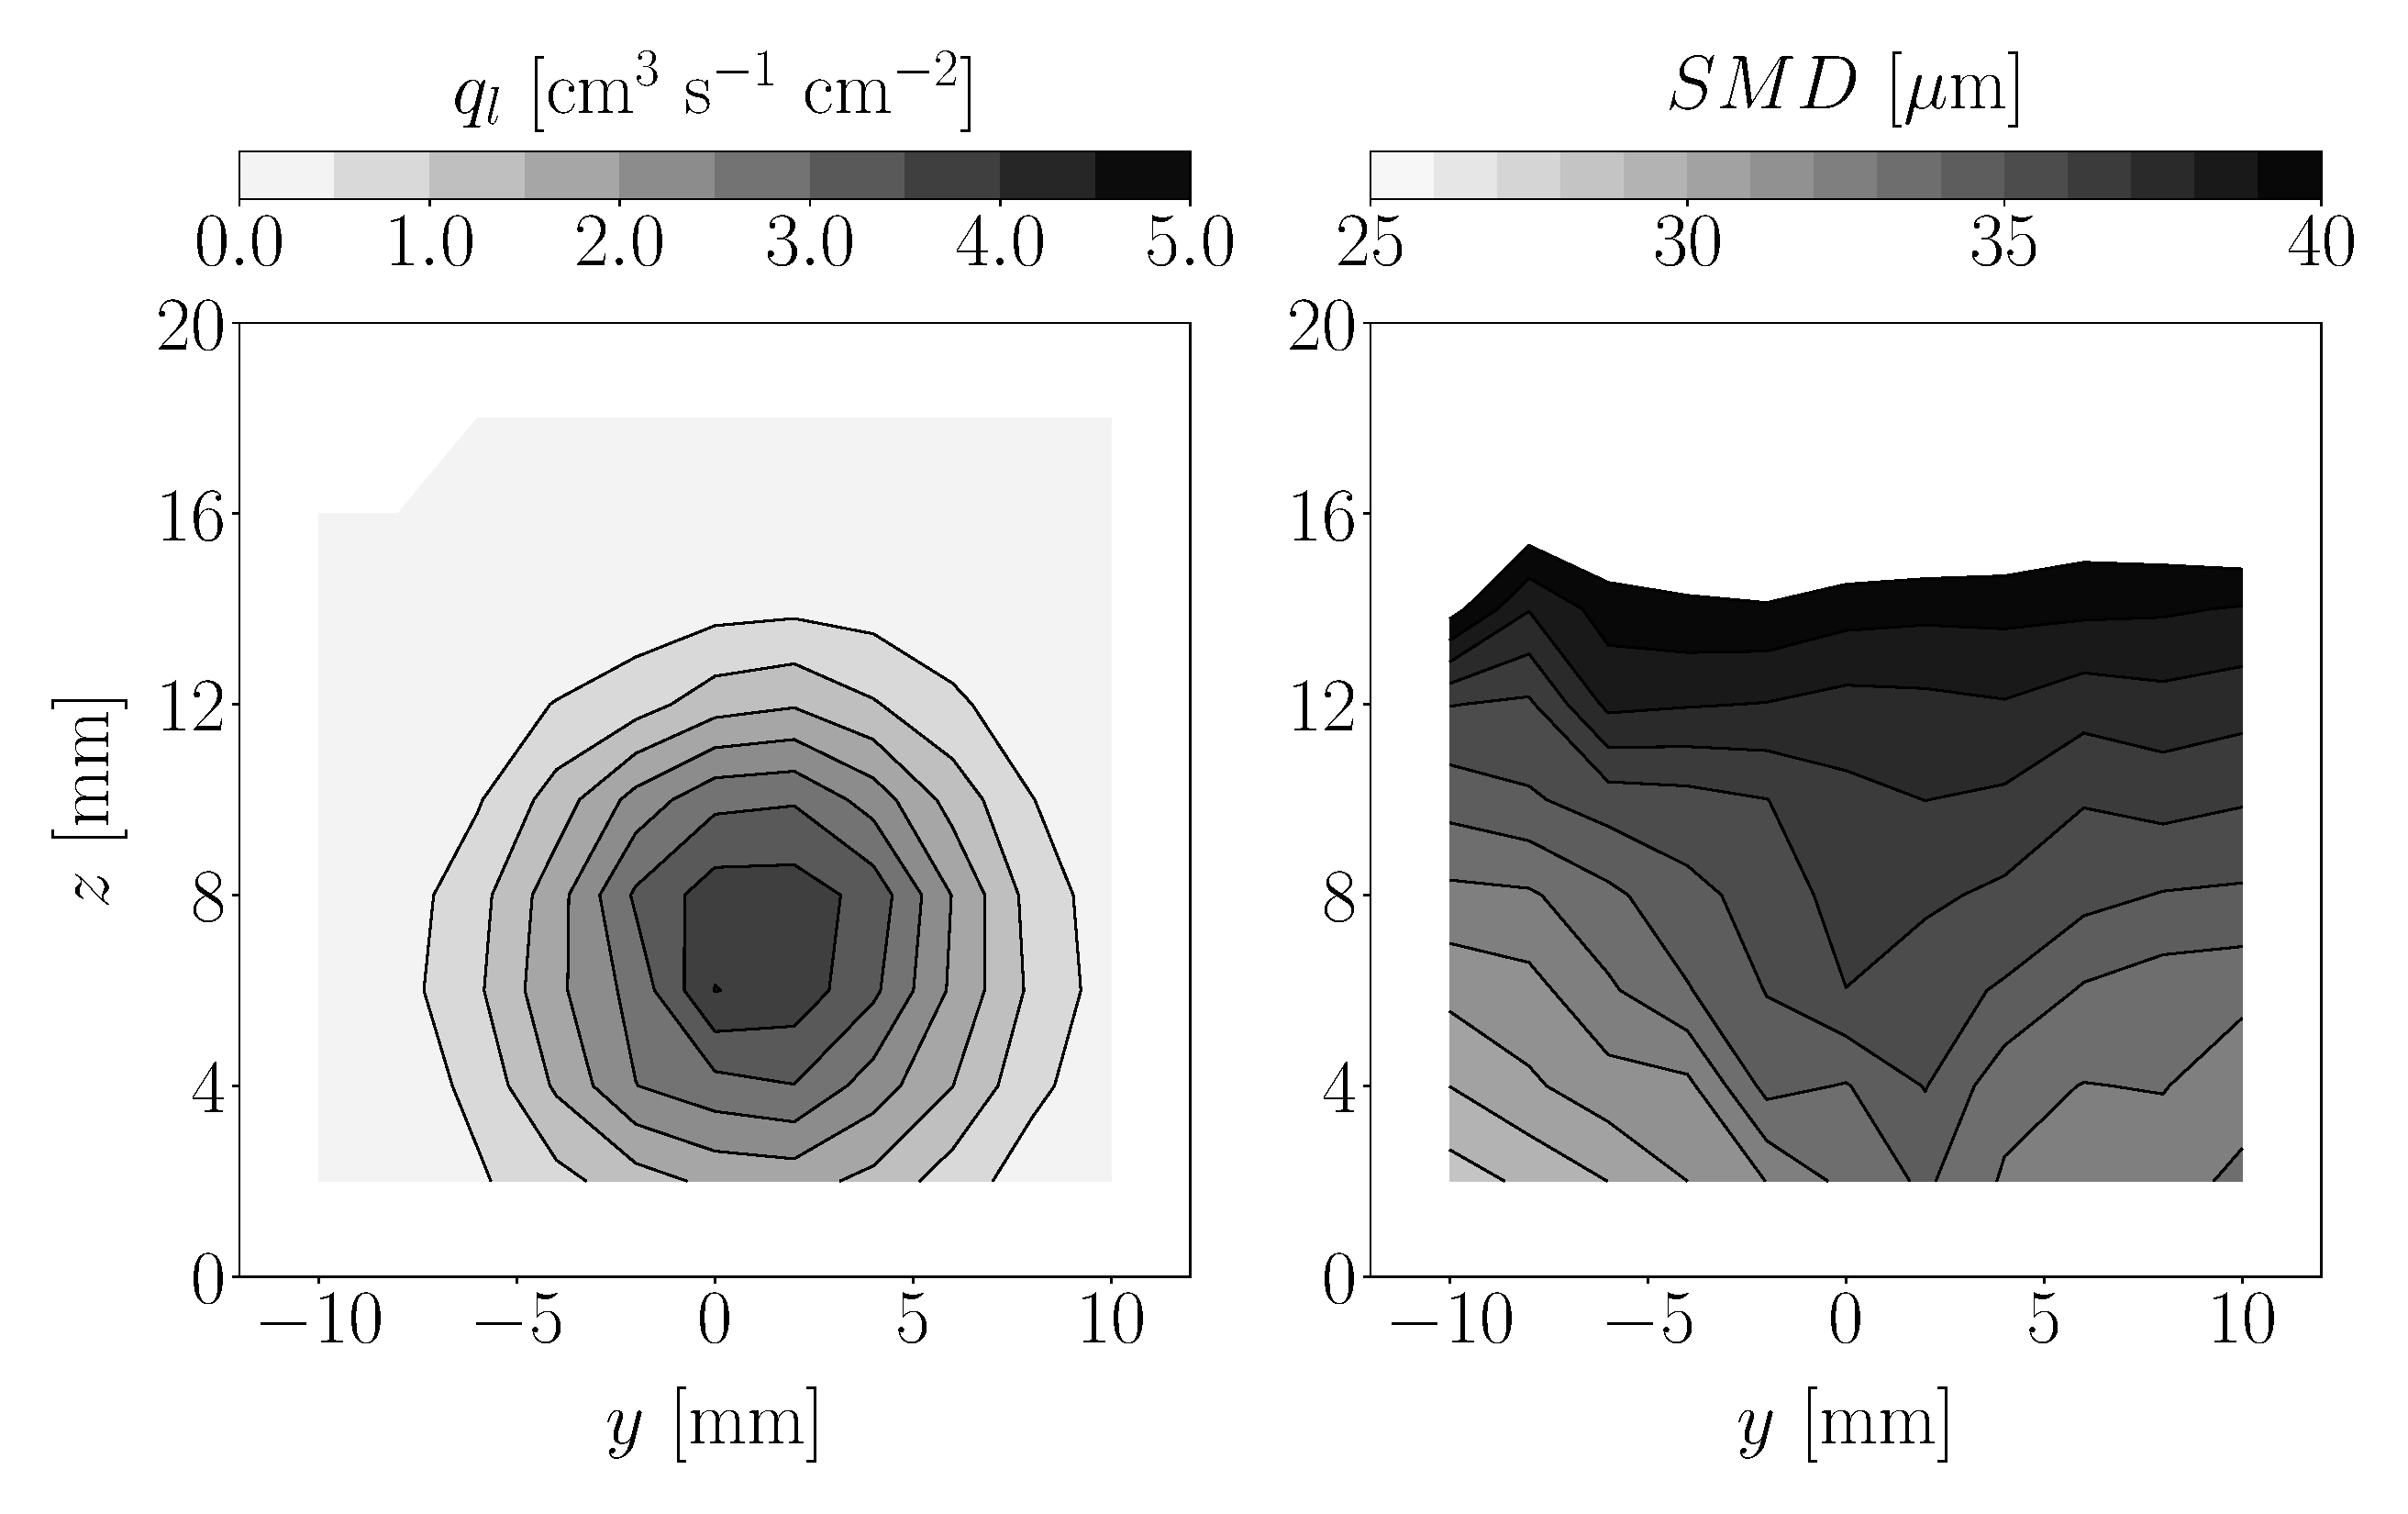
\includegraphics[scale=0.185]{./part2_developments/figures_ch6_lagrangian_JICF/expe_results/maps_UG75}
   \caption{Low Weber number operating point.}
   %\label{} 
\end{subfigure}
\hspace{0.3in}
\begin{subfigure}[b]{0.45\textwidth}
	\centering
   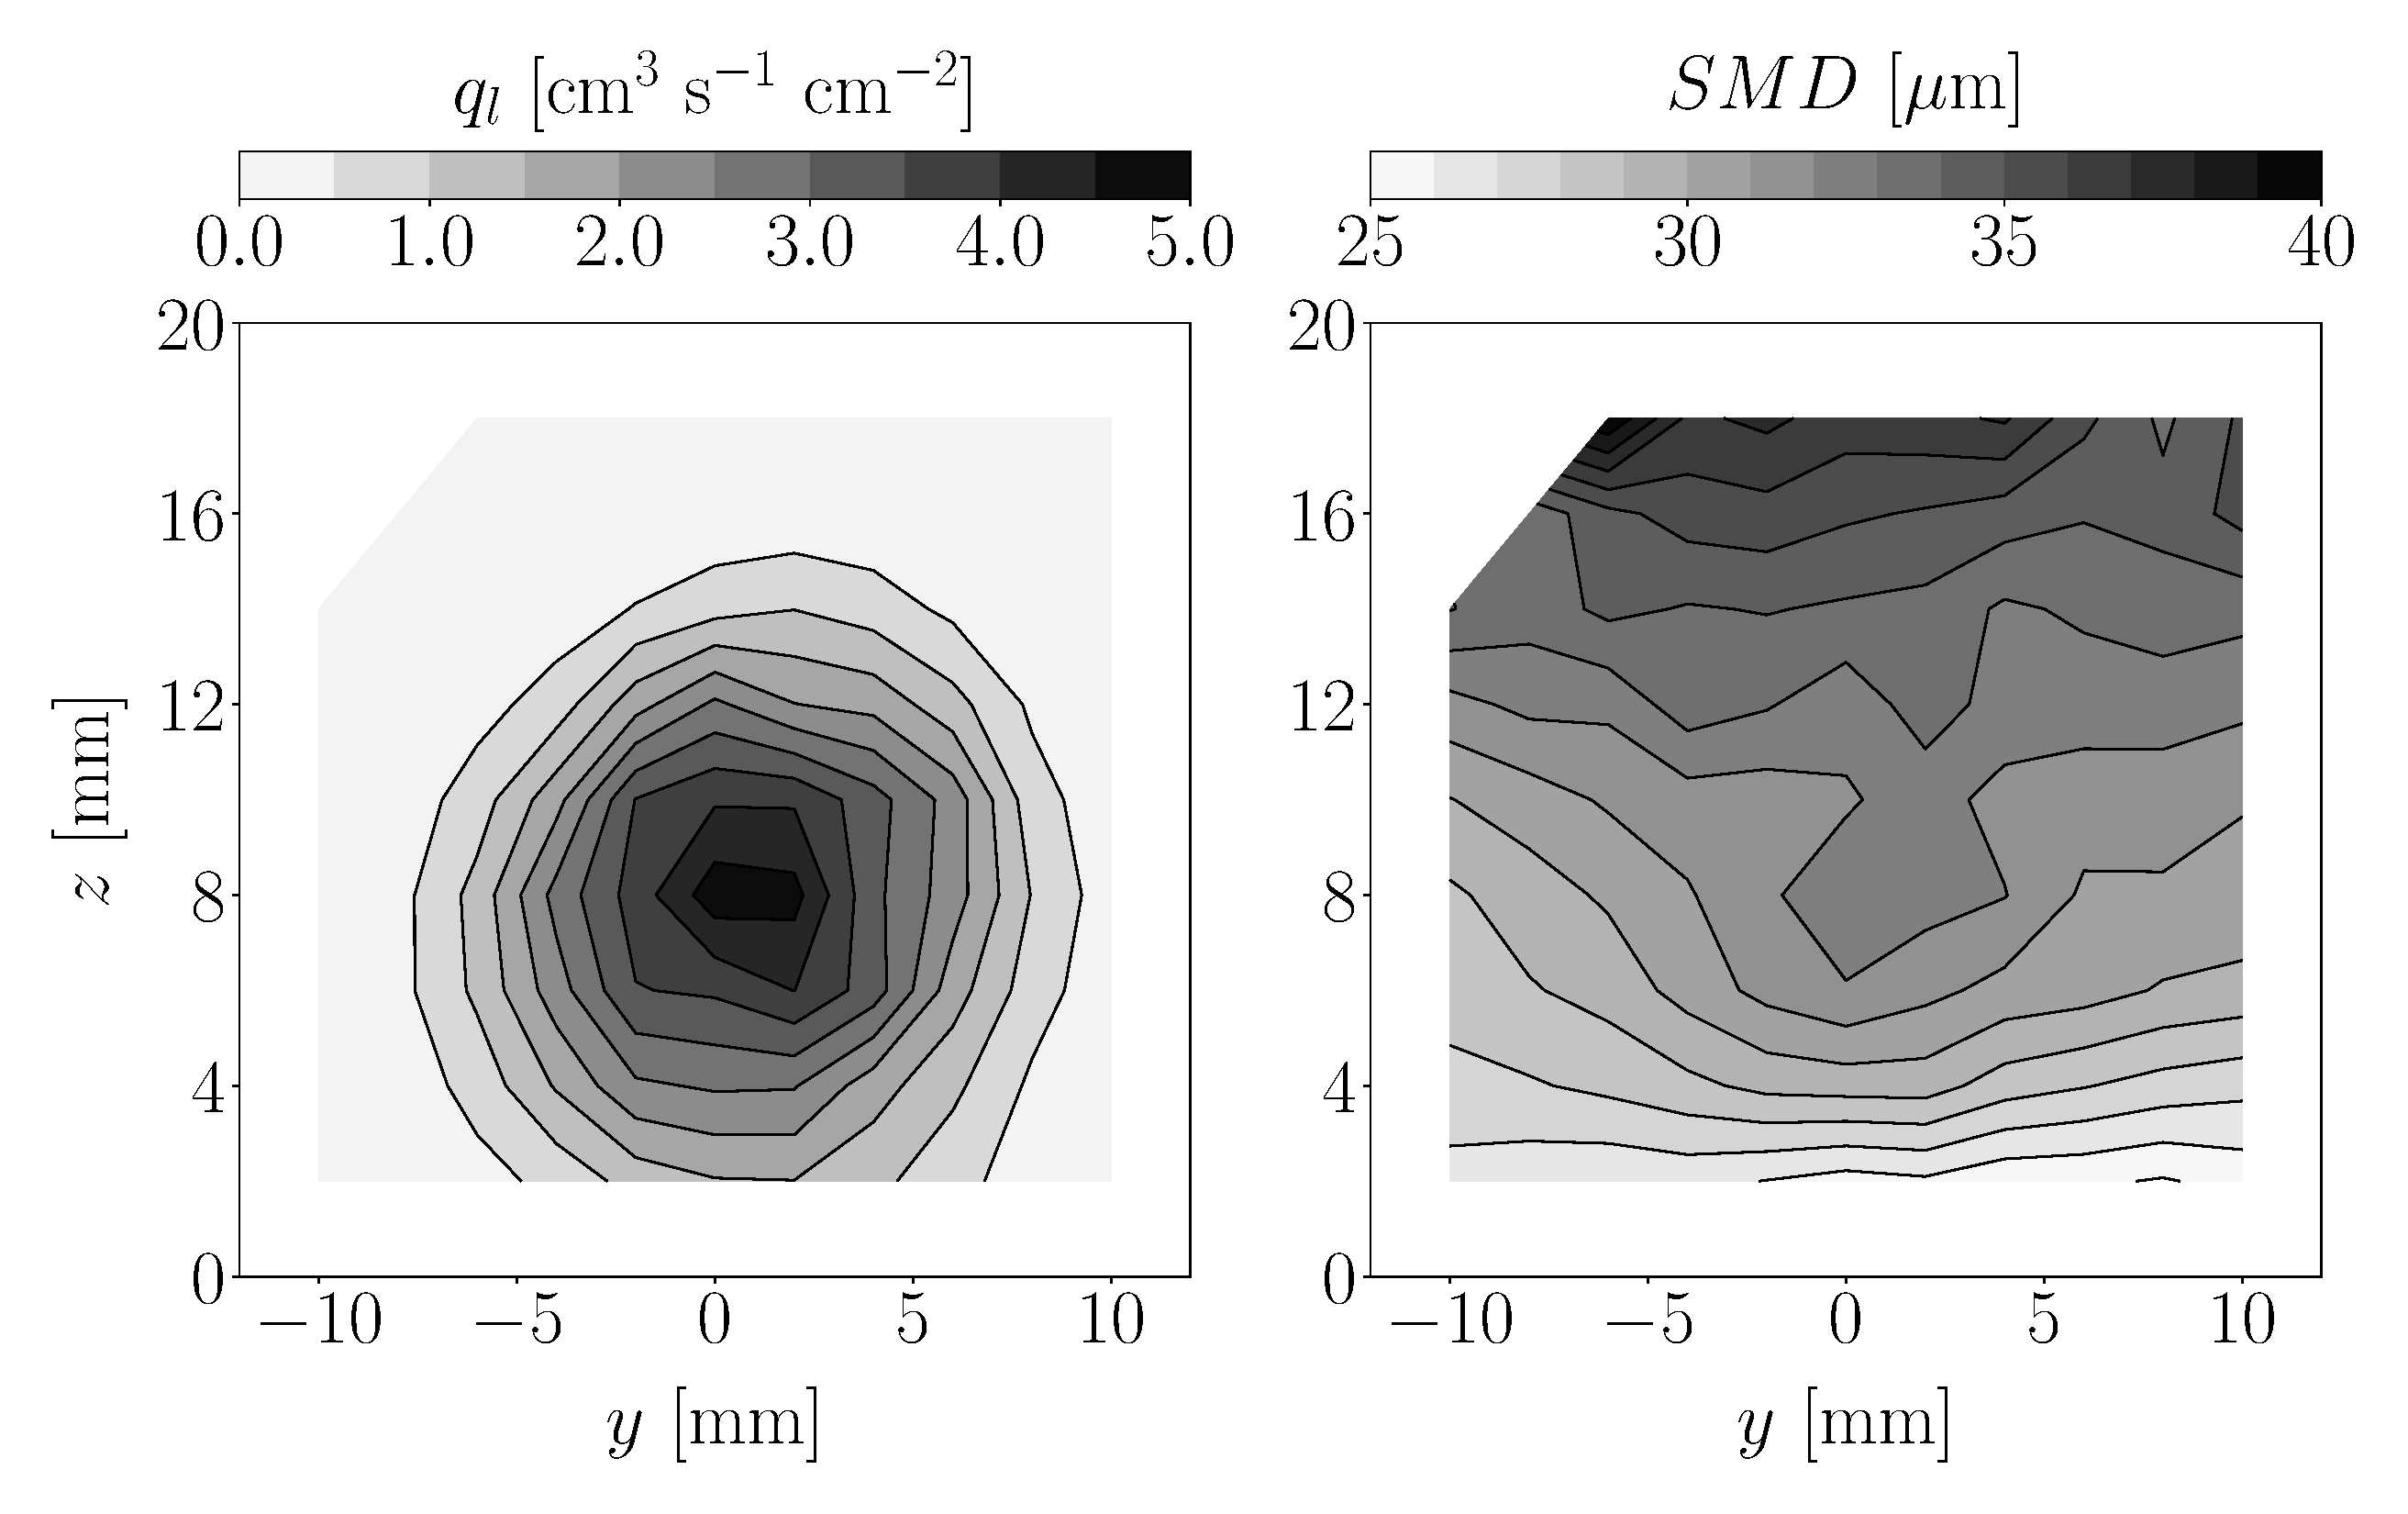
\includegraphics[scale=0.19]{./part2_developments/figures_ch6_lagrangian_JICF/expe_results/maps_UG100}
   \caption{High Weber number operating point.}
   %\label{} 
\end{subfigure}
\caption{SMD and volume flux maps obtained experimentally by \citeColor[becker_breakup_2002] at a location $x = 80$ mm downstream the liquid injector.}
\label{fig:maps_Becker_expe_results}
\end{figure}

Complementary to the maps, qualitative results are also present in the literature which can also be used for validation. These ones are given as the integrated profiles of the liquid volume flux and flux-averaged $SMD$ over the $z$ and $y$ directions, which are then respectively dependent on $y$ and $z$. The equations to obtain such measures are given by Eqs. (\ref{eq:integrated_results_Becker_expe_results}):


\begin{subequations}
\label{eq:integrated_results_Becker_expe_results}
\begin{align}
\langle q_l \left( z \right) \rangle = \frac{1}{L_y} \int_0^{L_y} q_l \left( y, z \right) dy    & ~~~~  ; & \langle SMD \left( z \right) \rangle = \frac{1}{L_y \langle q_l \left( z \right) \rangle} \int_0^{L_y} q_l \left( y, z \right) SMD \left( y, z \right) dy \\
\langle q_l \left( y \right) \rangle = \frac{1}{L_z} \int_0^{L_z} q_l \left( y, z \right) dz    & ~~~~  ; & \langle SMD \left( y \right) \rangle =  \frac{1}{L_z \langle q_l \left( z \right) \rangle} \int_0^{L_z} q_l \left( y, z \right) SMD \left( y, z \right) dz
\end{align}
\end{subequations}

%\begin{equation}
%\langle q_l \left( z \right) \rangle = \frac{1}{L_y} \int_0^{L_y} q_l \left( y, z \right) dy ~~~~; ~~~~ \langle SMD \left( z \right) \rangle = \frac{1}{L_y \langle q_l \left( z \right) \rangle} \int_0^{L_y} q_l \left( y, z \right) SMD \left( y, z \right) dy
%\end{equation}
%
%\begin{equation}
%\langle q_l \left( y \right) \rangle = \frac{1}{L_z} \int_0^{L_z} q_l \left( y, z \right) dz ~~~~; ~~~~ \langle SMD \left( y \right) \rangle = \frac{1}{L_z \langle q_l \left( z \right) \rangle} \int_0^{L_z} q_l \left( y, z \right) SMD \left( y, z \right) dz
%\end{equation}

The application of these equations to the experimental results yield the curves from Figure \ref{fig:integrated_results_Becker_expe_results}. The integrated volume flux over $y$ (Figure \ref{fig:integrated_results_Becker_expe_results_over_y}) shows an increase of the volume flux from the bottom part of the spray (PDA measurements closer to wall, for $z < 2$ mm, could not be performed \citeColor[becker_breakup_2002]) until the spray center, where the maximum flux is reached. Then, the flux decreases with $z$ until there is no more liquid present. Flux values are generally larger for the high $We$ point than for the low $We$ one, and the quantity of liquid extends up to further upstream for the former than for the latter due to its larger liquid velocity at injection. Regarding the SMD profiles, both cases follow a ballistic behaviour. The spray of the high $We$ point contains droplets of larger mean size than the low $We$ one.

With respect to the profiles integrated over $z$ (Figure \ref{fig:integrated_results_Becker_expe_results_over_z}), both SMD and flux lines follow parabollic profiles with the largest values present at $y = 0$, i.e. the coordinate for which the largest fluxes are found. The behaviour of the profiles depending on the operating point follow the same tendencies than in Figure \ref{fig:integrated_results_Becker_expe_results_over_y}: lower fluxes and larger droplets for the low $We$ case.



\begin{figure}[h!]
\flushleft
\begin{subfigure}[b]{0.45\textwidth}
	\flushleft
   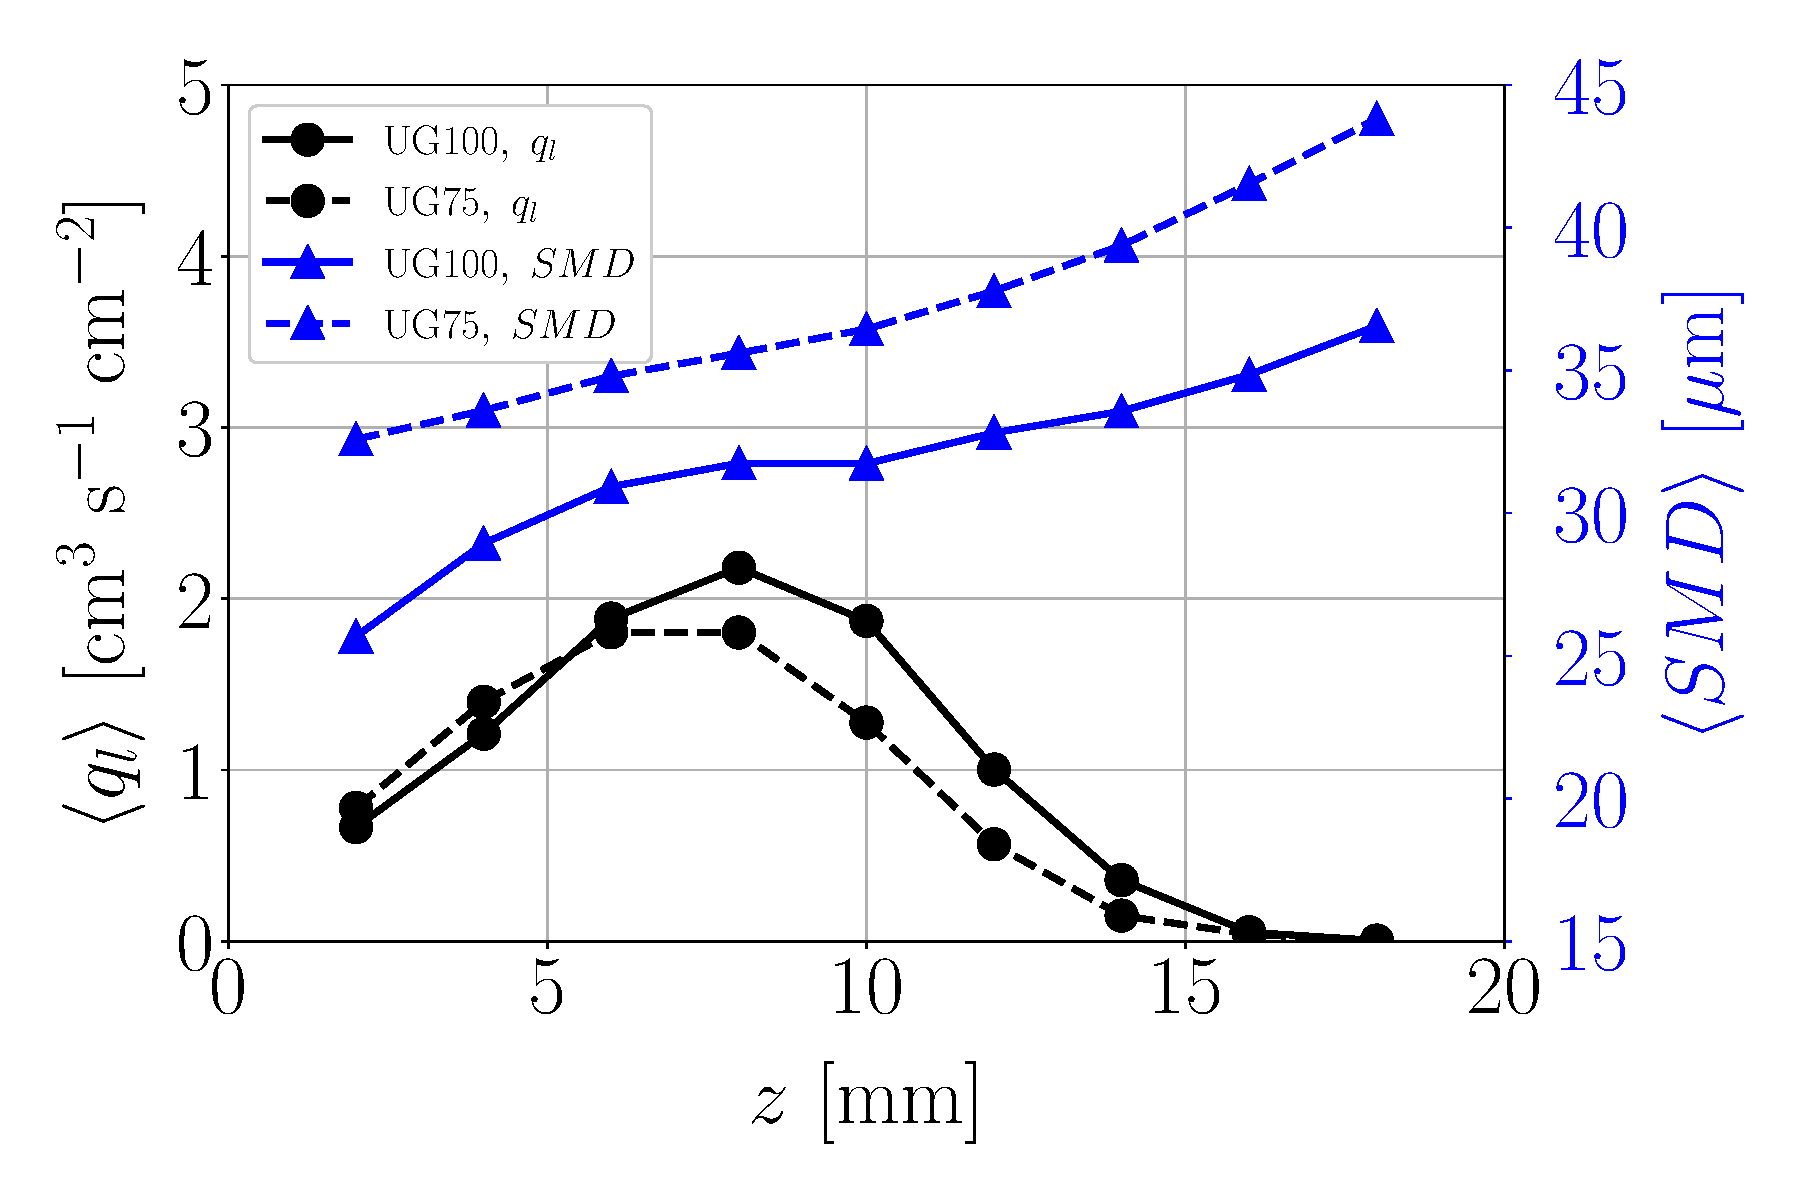
\includegraphics[scale=0.275]{./part2_developments/figures_ch6_lagrangian_JICF/expe_results/integrated_fluxes_along_y}
   \caption{Profiles integrated over $y$.}
  \label{fig:integrated_results_Becker_expe_results_over_y} 
\end{subfigure}
\hspace{0.3in}
\begin{subfigure}[b]{0.45\textwidth}
	\centering
   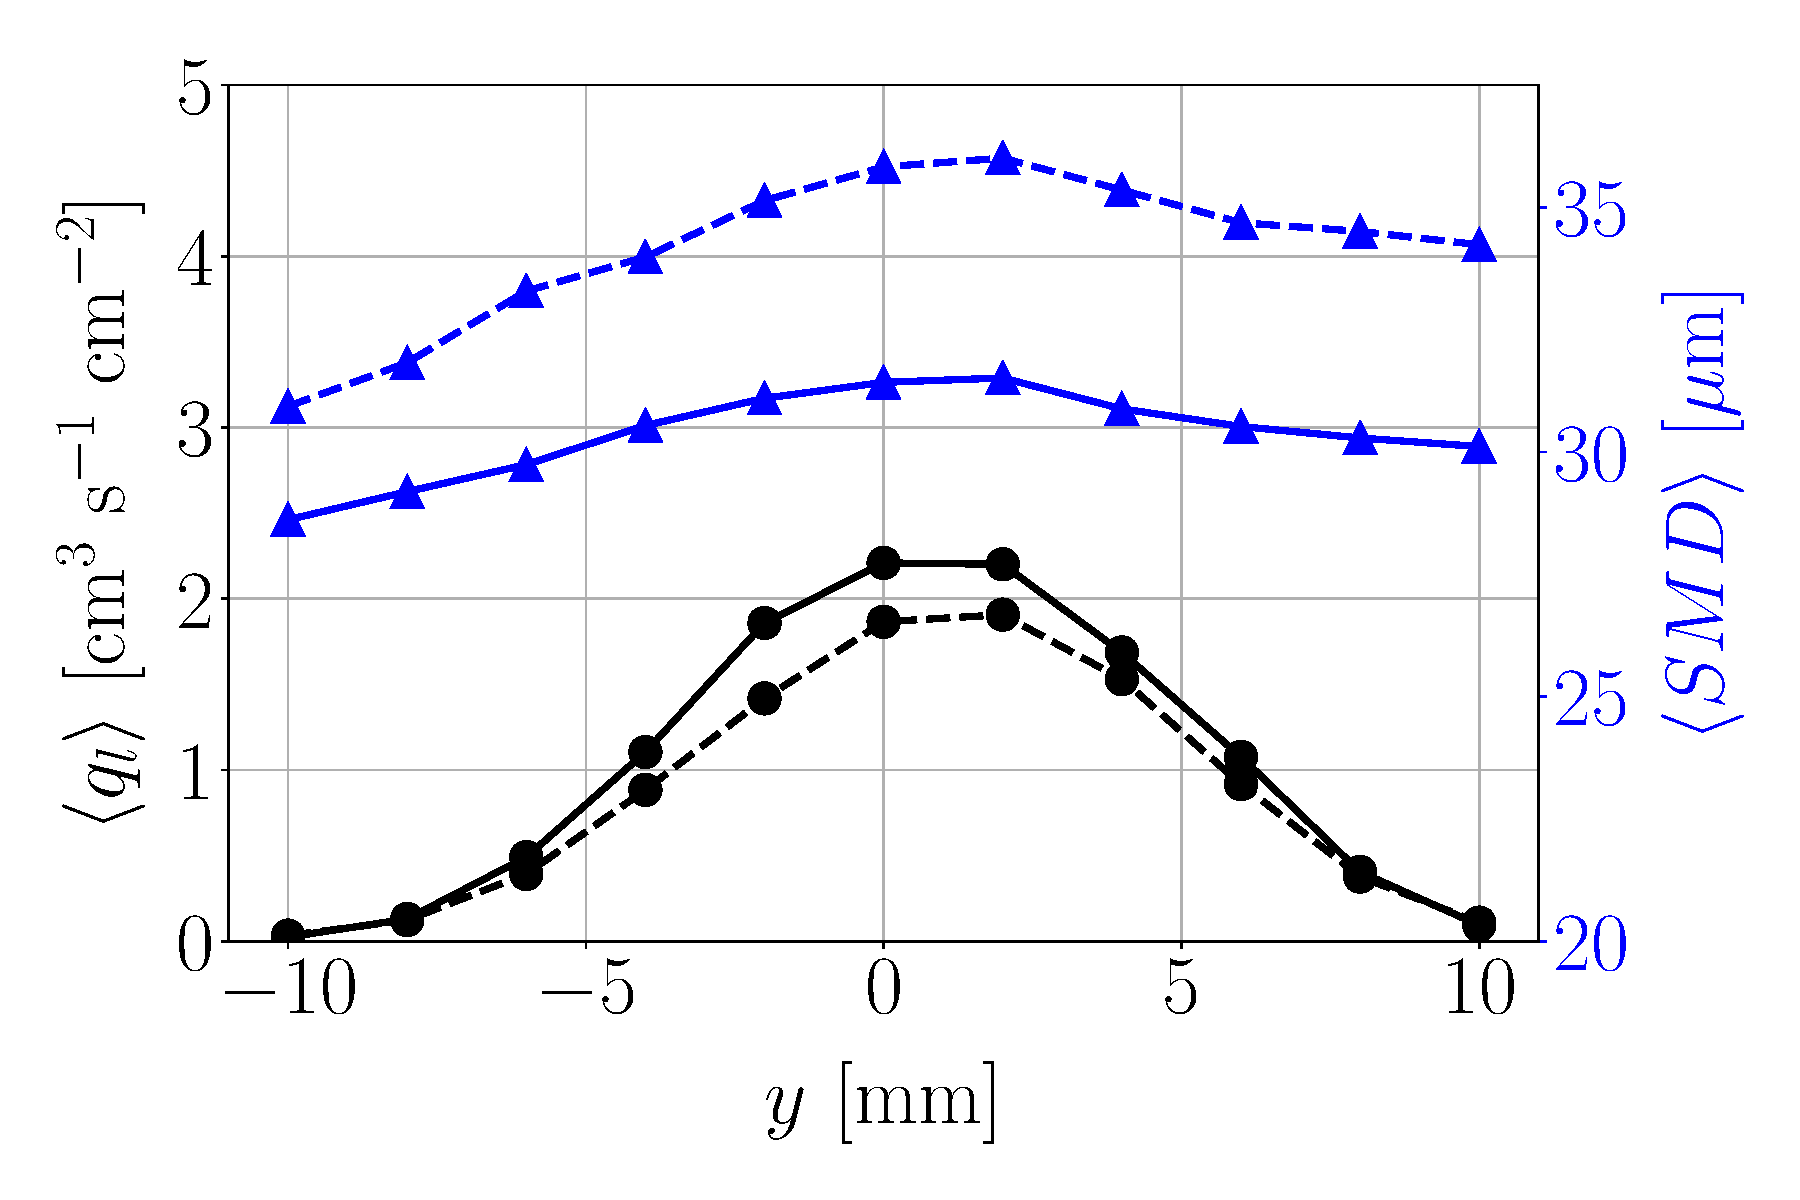
\includegraphics[scale=0.275]{./part2_developments/figures_ch6_lagrangian_JICF/expe_results/integrated_fluxes_along_z}
   \caption{Profiles integrated over $z$.}
  \label{fig:integrated_results_Becker_expe_results_over_z}
\end{subfigure}
\caption[{Integrated liquid volume flux and SMD profiles by \citeColor[becker_breakup_2002] at a location $x = 80$ mm downstream the liquid injector.}]{Integrated liquid volume flux and SMD profiles by \citeColor[becker_breakup_2002] at a location $x = 80$ mm downstream the liquid injector. }
\label{fig:integrated_results_Becker_expe_results}
\end{figure}

\section{Obtention of initial conditions with ALM}

Prior to liquid injection, it is necessary to establish an initial solution for the gaseous phase as done for the resolved simulations. The difference with respect to the resolved simulations is that in this case, the initial solutions needs to consider the ALM since the dense core blockage effect needs to be modelled in the dispersed phase simulations. All the details of the model were addressed in $\S$\ref{sec:ch4_dense_core_modelling}. In this section, firstly results from the resolved simulations are employed as input parameters to feed the ALM model. Secondly, gaseous simulations are performed with the ALM to obtain initial solutions. The resulting gaseous fields are compared to the ones of the resolved simulations to check the accuracy of the proposed actuator model. \\

%\subsection{Setup of actuator model}

The model parameters for ALM were described in Table \ref{tab:alm_parameters}. For the two operating points simulated, the corresponding input parameters are summarized in Table \ref{tab:jicf_lgs_ALM_parameters}. The points $x_b$, $z_b$ and $c_L$ are obtained from the mean values of Figure \ref{fig:dense_core_mean_parameters_scatterplots} for the fine simulations (note that $c_L$ is equivalent to the resolved dense core width $w$); $c_0$ is equal to the injector diameter; $N_p$ has been set to 20 as default, but it has been checked not to have an effect on the results; and the force $\textbf{F}_\mathrm{DC}$ is obtained as explained in $\S$\ref{ch5:subsec_defining_pressure_differences}.

\begin{table}[!h]
\centering
\caption{Parameters of an actuator representing the dense core}
\begin{tabular}{cccc}
\thickhline
\textbf{Parameter} & \textbf{Units} & \textbf{Low Weber} &  \textbf{High Weber} \\
\thickhline
$x_b$ & mm & & \\
$z_b$ & mm & & \\
$c_0$ & mm & 0.45 & 0.45 \\
$c_L$ & mm & & \\
$N_p$ & - & 20 & 20 \\
$| \textbf{F}_\mathrm{DC} |$ & N &  & \\
%$\Delta p$ & Pa &  & \\
\thickhline
\end{tabular}
\label{tab:jicf_lgs_ALM_parameters}
\end{table}

An example of an actuator representing the dense core in gaseous simulations \hl{can be seen in Figure }. As observed, it is graphically represented as a cylinder with the initial point located in the injection nozzle exit and final point in the breakup location of the resolved dense core estimated from the resolved simulations. The actuator points (not shown in the figure) are located uniformly along the central line of the cylinder. The discrete forces applied to each point are then mollified in the neighbouring cells in order to avoid flow singularities.

\subsection{Comparison between resolved and ALM gaseous fields}

The perturbed gaseous fields created by the presence of the dense core in the \hl{resolved simulations were discussed in $\S$}\ref{ch5:subsec_turbulent_structures_in_gaseous_field}. In the same fashion, equivalent postprocessings can be performed for the gaseous flow field 

A quantitative assessment of the actuator blockage effect can be performed by looking at the mean velocity distribution along the lines \textbf{XX} shown in Figure \ref{XX}. Equivalent data was obtained for the resolved simulations in \hl{\textbf{$\S$XX}}, which is also shown in the same Figure for comparison ... \\

OJO: ver pilotage 2021-05-26 para graficas de interes.

\subsection{Parametric study on actuator model}


\clearpage

\section{Effect of injection variables}

\hl{ALSO: effect of one and two-way coupling !! Ver articulos 2010, 2011 Li }.

\subsection{Design of experiments}

In Chapter \ref{ch5:jicf_resolved_simulations}, the five resolved atomization simulations from Table \ref{fig:location_JICF_ops_in_breakup_map} were performed and analyzed. These ones tested two mesh interface mesh resolutions ($\Delta x_\mathrm{min} = 20, 10~\mu$m), two operating points ($We_g = 830, 1470$) and the influence of turbulence injection in one simulation for the coarse resolution, high $We_g$ case. Results shown a high dependency of the trajectories ($\S$\ref{subsec:ch5_jet_trajectories_results}) and jet topologies ($\S$\ref{sec:ch5_jet_evolution}) on the resolution, which led later to different spray characteristics ($\S$\ref{sec:ch5_sec_spray_characterization}) and resulting injectors ($\S$\ref{sec:ch5_learning_SLI}) for each case, which a high dependency on the operating point due to the different velocity magnitudes involved. Therefore, it is of interest to test such effects in the disperse-phase simulations by initializing these computations with the different injectors obtained.

Apart from the resolved simulation parameters (i.e. $\Delta x_\mathrm{min}$, operating condition, turbulence injection), the SLI parameters to perform injection derived in Chapter \ref{ch4:sli_development} and summarized in Table \ref{subsec:ch4_injectors_definition} can also be tested, as well as the influence of the ALM model ($\S$\ref{sec:ch4_dense_core_modelling}) and the secondary atomization models ($\S$\ref{sec:ch4_dense_core_modelling}). The influence of all these parameters can be studied by performing a design of experiments with consists of the simulations from Table \ref{tab:lgs_jicf_DoF}, and which proceeds as follows: 


\begin{itemize}

	\item A \textbf{baseline} case is selected to perform injection. The resolved case UG100\_DX10 is chosen with injection being performed at $x_\mathrm{inj} = 5$ mm, ALM activated, Gaussian $\textbf{r}$  law and Gorokhovski's atomization model ($\S$\ref{subsec:ch4_goro_model}). \hl{This case was studied in ... and has been selected because ...}. It corresponds to case 1 from Table \ref{tab:lgs_jicf_DoF}, and all the rest of dispersed-phase simulations are compared to this case.

		\item The effect of the \textbf{resolved mesh resolution} in the injectors is studied by keeping all parameters identical but choosing the SLI obtained from case UG100\_DX20 (see Figure \textbf{XX}). It corresponds to case 2 from Table \ref{tab:lgs_jicf_DoF}

	\item The effect of \textbf{injection location} $x_\mathrm{inj}$ downstream the injector nozzle. The resolved JICF trajectories from Figure \ref{fig:JICF_trajectories_validation} show that the numerical trajectories are properly estimated in the near-nozzle region but that after a certain point, the coarse resolutions underestimate the trajectory while the fine ones overestimate it. To study the influence this can have in the dispesed-phase simulations, three different simulations are performed: two simulations for the resolved case UG100\_DX10 at 1) $x = 5$ mm ($x/d_\mathrm{inj} = 11$);, where the trajectory is properly estimated, and 2) $x = 10$ mm ($x/d_\mathrm{inj} = 22$) where the trajectory is overestimated; and 3) one simulation for the resolved case UG100\_DX20 at $x = 10$ mm ($x/d_\mathrm{inj} = 22$), where the trajectory is underestimated. These cases have been considered since they present low relative values for mass conservation of liquid mass, as shown in Figure \ref{fig:delta_Ql_with_x}. Both simulations performed correspond to cases 3 and 4 from Table \ref{tab:lgs_jicf_DoF}.
	
	\item The \textbf{operating condition} is tested by simulating the case UG75\_DX10 with the rest of parameters identical to the baseline (case 5 from Table \ref{tab:lgs_jicf_DoF}).
	
	\item \hl{The effect of the \textbf{injection diameters law} $f_0$ ...}
	
	\item \textbf{Spray velocities in the SLI} are tested by simulating the baseline case with the two other $\text{r}$ laws: uniform and zero, corresponding to cases 6 and 7 from Table \ref{tab:lgs_jicf_DoF}.
	
	\item A simulation without \textbf{ALM} is performed (case 8 from Table \ref{tab:lgs_jicf_DoF}).
	
	\item Finally, the effect of the different atomization models is tested by using the TAB and ETAB modes with the baseline conditions (cases 9 and 10 from Table \ref{tab:lgs_jicf_DoF}).	
	
\end{itemize}

\clearpage
	
%\begin{table}[!h]
%\centering
%\caption{Design of experiments to test injection parameters. Modified parameters are highlighted in blue.}
%\begin{tabular}{ccccccc}
%\thickhline
%\multirow{2}{*}{ \textbf{Case}} &  \multirow{2}{*}{ \begin{tabular}{c} \textbf{Resolved} \\ \textbf{simulation} \end{tabular}}    &  \multirow{2}{*}{  \begin{tabular}{c} $x_\mathrm{inj}$  \\ $\left[ \mathrm{mm} \right]$ \end{tabular}} &   \multirow{2}{*}{ \begin{tabular}{c} $\textbf{r}$ \\ \textbf{law} \end{tabular}} & \multirow{2}{*}{ \textbf{ALM ?}}  & \multirow{2}{*}{ \begin{tabular}{c} \textbf{Atomization} \\ \textbf{model} \end{tabular}} &    \multirow{2}{*}{ \textbf{Description}}\\
% & & & & & & \\
%\thickhline
%\vspace*{0.1in}
%1 & UG100\_DX10 & 5 & Gaussian & Yes & Goro  & Baseline \tab_space
%\multirow{2}{*}{2} & \multirow{2}{*}{UG100\_\textcolor{blue}{DX20}} & \multirow{2}{*}{5} & \multirow{2}{*}{Gaussian} & \multirow{2}{*}{Yes} & \multirow{2}{*}{Goro}  &  
% \multirow{2}{*}{ \begin{tabular}{c} Effect of \\ resolution \end{tabular}} \\
% & & & & & & \tab_space
%3 & UG100\_DX10 & \textcolor{blue}{10} & Gaussian & Yes & Goro  & Effect of $x_\mathrm{inj}$ \tab_space
%4 & UG100\_\textcolor{blue}{DX20} & \textcolor{blue}{10} & Gaussian & Yes & Goro  & Effect of $x_\mathrm{inj}$ \tab_space
%\multirow{2}{*}{5} & \multirow{2}{*}{\textcolor{blue}{UG75}\_DX10} & \multirow{2}{*}{10} & \multirow{2}{*}{Gaussian} & \multirow{2}{*}{Yes} & \multirow{2}{*}{Goro}  & \multirow{2}{*}{ \begin{tabular}{c} Effect of  \\ operating condition  \end{tabular}} \\
% & & & & & & \tab_space
%6 & UG100\_DX10 & 5 & \textcolor{blue}{Uniform} & Yes & Goro  & Effect of $r$ law \tab_space
%7 & UG100\_DX10 & 5 & \textcolor{blue}{Zero} & Yes & Goro  & Effect of $r$ law \tab_space
%8 & UG100\_DX10 & 5 & Gaussian & \textcolor{blue}{No} & Goro  & Effect of ALM \tab_space
%\multirow{2}{*}{9} & \multirow{2}{*}{UG100\_DX10} & \multirow{2}{*}{5} & \multirow{2}{*}{Gaussian} & \multirow{2}{*}{Yes} & \multirow{2}{*}{\textcolor{blue}{TAB}} & \multirow{2}{*}{ \begin{tabular}{c} Effect of  \\ atomization model\end{tabular}}\\
% & & & & & & \tab_space
%\multirow{2}{*}{10} & \multirow{2}{*}{UG100\_DX10} & \multirow{2}{*}{5} & \multirow{2}{*}{Gaussian} & \multirow{2}{*}{Yes} & \multirow{2}{*}{\textcolor{blue}{ETAB}} & \multirow{2}{*}{ \begin{tabular}{c} Effect of  \\ atomization model\end{tabular}}\\
% & & & & & & \tab_space
%\thickhline
%\end{tabular}
%\label{tab:lgs_jicf_DoF}
%\end{table}

	
\begin{table}[!h]
\centering
\caption{Design of experiments to test injection parameters. Blue color indicates modified parameters.}
\begin{tabular}{ccccccc}
\thickhline
\multirow{2}{*}{ \textbf{Case}} &  \multirow{2}{*}{ \begin{tabular}{c} \textbf{Resolved} \\ \textbf{simulation} \end{tabular}}    &  \multirow{2}{*}{  \begin{tabular}{c} $x_\mathrm{inj}$  \\ $\left[ \mathrm{mm} \right]$ \end{tabular}} &   \multirow{2}{*}{ \begin{tabular}{c} $\textbf{r}$ \\ \textbf{law} \end{tabular}} & \multirow{2}{*}{ \textbf{ALM ?}}  & \multirow{2}{*}{ \begin{tabular}{c} \textbf{Atomization} \\ \textbf{model} \end{tabular}} &    \multirow{2}{*}{ \textbf{Modification}}\\
 & & & & & & \\
\thickhline
1 & UG100\_DX10 & 5 & Gaussian & Yes & Goro  & Baseline \tab_space
2 & UG100\_\textcolor{blue}{DX20} & 5 & Gaussian & Yes & Goro  & SPS resolution \tab_space
3 & UG100\_DX10 & \textcolor{blue}{10} & Gaussian & Yes & Goro  & $x_\mathrm{inj}$ \tab_space
4 & UG100\_\textcolor{blue}{DX20} & \textcolor{blue}{10} & Gaussian & Yes & Goro  & $x_\mathrm{inj}$ \tab_space
5 & \textcolor{blue}{UG75}\_DX10 & 10 & Gaussian & Yes & Goro  & Operating condition \tab_space
6 & UG100\_DX10 & 5 & \textcolor{blue}{Uniform} & Yes & Goro  & $r$ law \tab_space
7 & UG100\_DX10 & 5 & \textcolor{blue}{Zero} & Yes & Goro  & $r$ law \tab_space
8 & UG100\_DX10 & 5 & Gaussian & \textcolor{blue}{No} & Goro  & ALM \tab_space
9 & UG100\_DX10 & 5 & Gaussian & Yes & \textcolor{blue}{TAB} & Atomization model \tab_space
10 & UG100\_DX10 & 5 & Gaussian & Yes & \textcolor{blue}{ETAB} & Atomization model \tab_space
\thickhline
\end{tabular}
\label{tab:lgs_jicf_DoF}
\end{table}

	
\subsection{Results}

\subsubsection*{Effect of mesh resolution}

\subsubsection*{Effect of injection location}

\subsubsection*{Effect of operating condition}

\subsubsection*{Effect of $\textbf{r}$ law}

\subsubsection*{Effect of ALM}

\subsubsection*{Effect of atomization model}


\clearpage


\section{Relation between volume and mixture fractions}

So we can relate $\overline{\alpha}$ field with the mixture fraction somehow, this will be interesting for people doing combustion. I have developed the following relation between mixture fraction $Z$ and volume fraction $\alpha$ (need to check it properly):

\begin{equation}
Z = \frac{m_l}{m_l + m_g} = \frac{V_l \rho_l}{V_l \rho_l + V_g \rho_g} = \frac{1}{1 + \frac{V_g}{V_l} \frac{\rho_g}{\rho_l}} = \frac{1}{1 + \frac{\rho_g}{\rho_l} \frac{1 - \alpha}{\alpha}}
\end{equation}


We can also make a link to heat relase, for the interest of combustion studies.




\section{Results}

\subsection{Mesh convergence study}

\subsection{Validation with experiments (quantitative/qualitative)}

\subsection{Trajectories}

In order to illustrate the lagrangian trajectories and the continuity with respect to the resolved jets, a volume fraction field can be defined in the lagrangian simulations:

\begin{equation}
\alpha_l \left( \textbf{x}, t \right) = \frac{V_l \left( \textbf{x}, t \right)}{V_{el}}
\end{equation}

where $V_{el}$ is the volume of the element in the eulerian mesh grid. Therefore, the volume fraction is a magnitude defined in the main eulerian grid. Since the dispersed phase is not directly represented in this grid but by lagrangian particles, $V_l \left( \textbf{x}, t \right)$ is calculated by interpolating the volume of the particles located within each element at each iteration.

\subsection{Frequential analysis}

Several probes have been located in the outer part of the jet to see the spectra. See Figures \ref{fig:probes_dx10m} and \ref{fig:probes_dx20m} for volume fraction probes, and Figure \ref{fig:probes_U_planey0} for determining velocity spectra at plane y = 0. These are available at pilotage 30-04-2021.

Para velocidades: OJITO con la probe 18 !

\begin{figure}[h!]
	\centering
	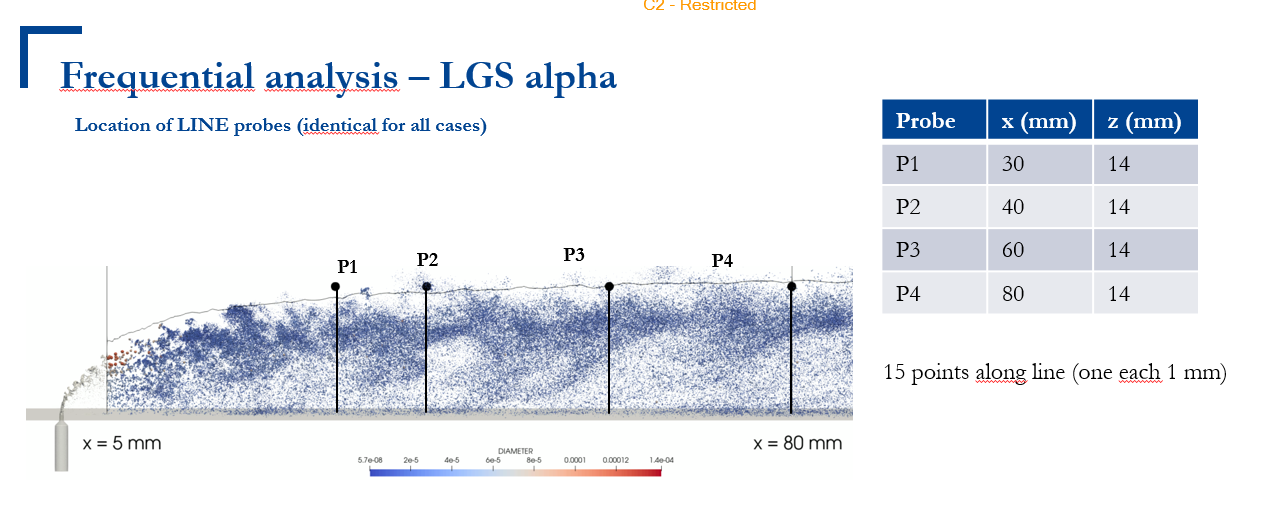
\includegraphics[scale=0.7]{./part2_developments/figures_ch6_lagrangian_JICF/probes_vol_frac}
	\caption{Probes for $\alpha$ frequential analysis for volume fraction}
	\label{fig:probes_dx10m}
\end{figure}


\begin{figure}[h!]
	\centering
	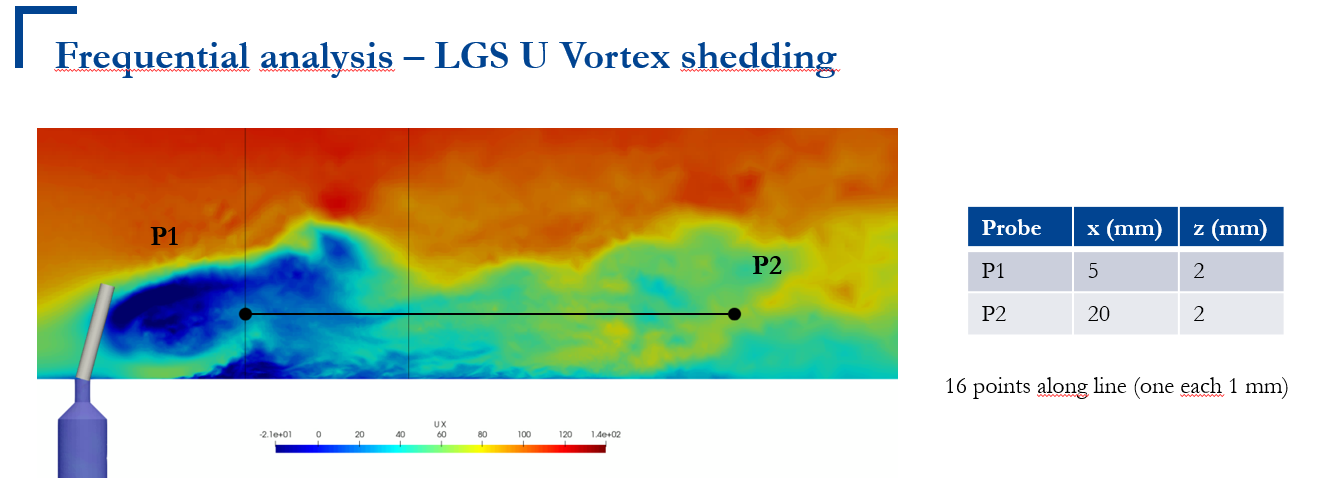
\includegraphics[scale=0.7]{./part2_developments/figures_ch6_lagrangian_JICF/probes_U_planey0}
	\caption{Probes for $U$ study}
	\label{fig:probes_U_planey0}
\end{figure}

\section{Performance of the simulations}

These ones are cheaper than the resolved ones.



\section{Conclusions}